\subsubsection{Modelo autoregresivo (AR)}\label{model_ar}


Un modelo autoregresivo es otro tipo de redes neuronal recurrente. Esta red tiene como peculiaridad que el resultado obtenido se usa como valor de entrada para el calculo de la siguiente iteración. El modelo generado gráficamente es el siguiente:
\begin{figure}[H]
    \centering
    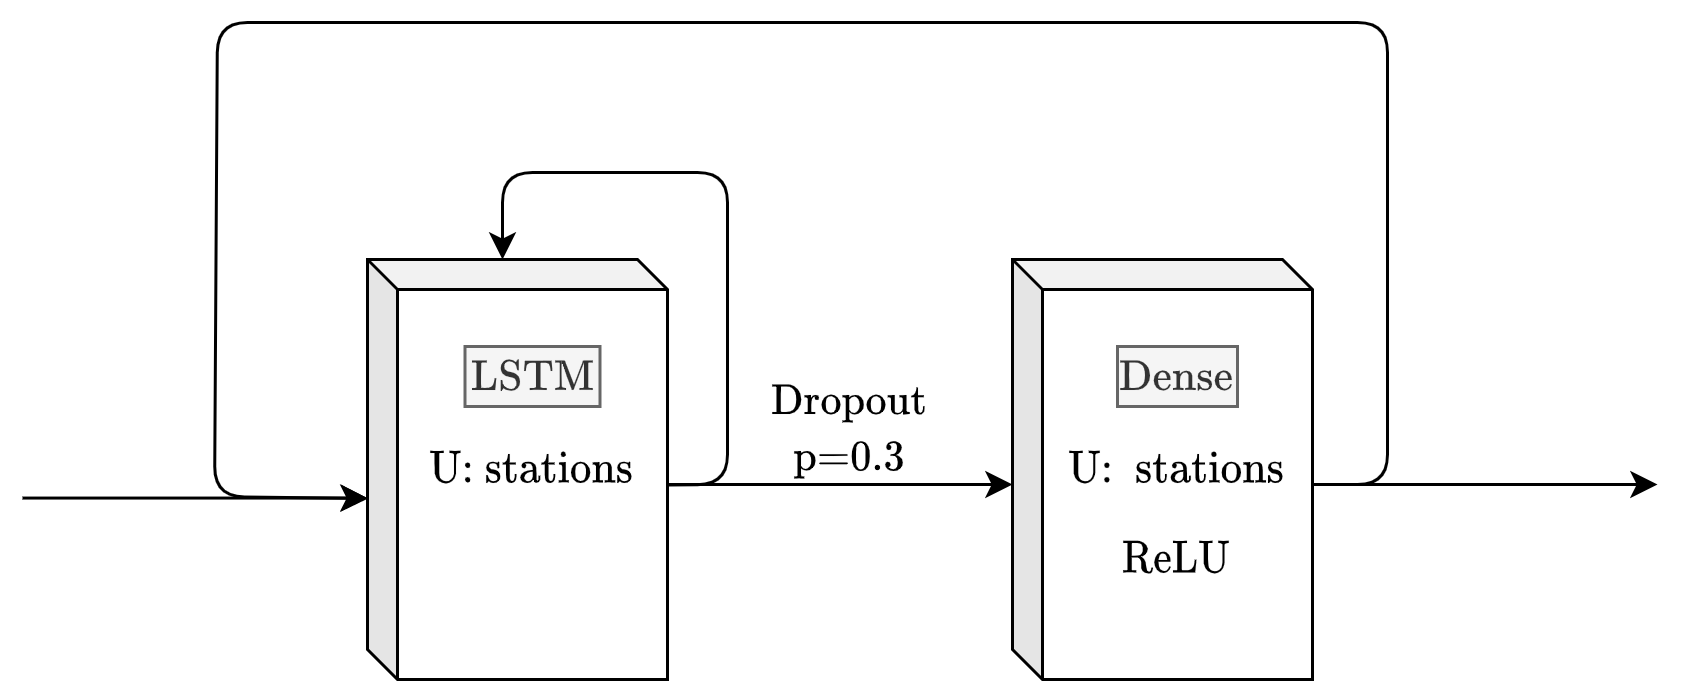
\includegraphics[width=10cm]{images/solution/models/AR.png}
    \caption{Modelo recurrente Autoregresivo}
    \label{fig:dense-model}
\end{figure}

El modelo tiene una capa LSTM junto con una capa densa. La salida de esta capa que es la predicción del modelo se reintroduce en el modelo para predecir el resto de predicciones.
\newline

\textit{Tensorflow} no dispone de un modelo en su librería que supliese las necesidades que buscábamos, por esa razón, se ha tenido que implementar este modelo usando otra técnica. Se ha creado una clase nueva que hereda de \small\verb|tf.keras.Model| y la cual tiene tres métodos: \small\verb|__init__|, \small\verb|warmup| y \small\verb|call|. De esta forma se pueden generar modelos que puedan tener arquitecturas singulares y distintas a las \textit{pass-forward}. Para la implementación se ha seguido la documentación de \textit{Tensorflow} \cite{tensorflow2015-whitepaper} y \textit{Keras} \cite{keras}.
\newline

La clase usada para definir el modelo autoregresivo ha sido el siguiente:
\begin{minted}[fontsize=\scriptsize]{python}
import tensorflow as tf
from tensorflow.keras.layers import LSTMCell, RNN, Dense

class AutoRegressive(tf.keras.Model):
    def __init__(self, lstm_units, steps, stations):
        super().__init__()
        self.steps = steps
        self.stations = stations
        self.lstm_units = lstm_units
        
        # First LSTM layer
        self.lstm_cell = LSTMCell(lstm_units)
        # Also wrap the LSTMCell in an RNN to simplify the `warmup` method.
        self.lstm_rnn = RNN(self.lstm_cell, return_state=True)
        
        # Ouput layer
        self.dense = Dense(stations, activation="relu")

    def warmup(self, inputs):
        # inputs.shape => (batch, time, features)
        # x.shape => (batch, lstm_units)
        x, *state = self.lstm_rnn(inputs)

        # predictions.shape => (batch, features)
        prediction = self.dense(x)
        return prediction, state

    def call(self, inputs, training=None):
        # Use a TensorArray to capture dynamically unrolled outputs.
        predictions = []

        # Initialize the lstm state
        prediction, state = self.warmup(inputs)

        # Insert the first prediction
        predictions.append(prediction)

        # Run the rest of the prediction steps
        for n in range(1, self.steps):
            # Use the last prediction as input.
            x = prediction
            
            # Concat with timestamp variables
            x = tf.concat([x, inputs[:,-1,-3:]], 1)
            
            # Execute one lstm step.
            x, state = self.lstm_cell(x, states=state, training=training)
                                      
            # Convert the lstm output to a prediction.
            prediction = self.dense(x)
            
            # Add the prediction to the output
            predictions.append(prediction)

        # predictions.shape => (time, batch, features)
        predictions = tf.stack(predictions)
        
        # predictions.shape => (batch, time, features)
        predictions = tf.transpose(predictions, [1, 0, 2])
        
        return predictions
\end{minted}


Para crear un nuevo modelo simplemente se genera una nueva instancia de la siguiente manera:
\begin{minted}[fontsize=\scriptsize]{python}
AutoRegressive(lstm_units=stations, steps=steps, stations=stations)
\end{minted}

Los resultados del modelo se pueden ver junto al resto de resultados en la sección \ref{results}.